\documentclass[fleqn, 10pt]{article}


\usepackage[utf8]{inputenc}
\usepackage{amsthm, amsmath}
\usepackage{nccmath} %Para centrar ecuaciones
\usepackage{graphicx}
\usepackage{enumitem}
\graphicspath{ {} } 

    \title{\textbf{Practica 4}}
    \author{Daniel García Villodres}
    \date{}
    
    \addtolength{\topmargin}{-3cm}
    \addtolength{\textheight}{3cm}
    

    
\begin{document}

\maketitle
\thispagestyle{empty}

\section*{Actividad 1}
Create the simplest WHILE program that computes the diverge function (with
zero arguments) and compute the codification of its code.

\subsection*{}

\begin{verbatim}
F("(1, X1=X1+1; while X1!=0 do X1=X1 od)", [0])
complexity has reached 1000, press Ctrl-C to stop, or any other key to continue...

CODE2N("X1:=X1+1;while X1!=0 do X1:=X1 od")
ans = 139126
\end{verbatim}


\section*{Actividad 2}
Create an Octave script that enumerates all the vectors.

\begin{verbatim}
i = 0
while (true)
  godeldecoding(i)
  i++
endwhile
\end{verbatim}
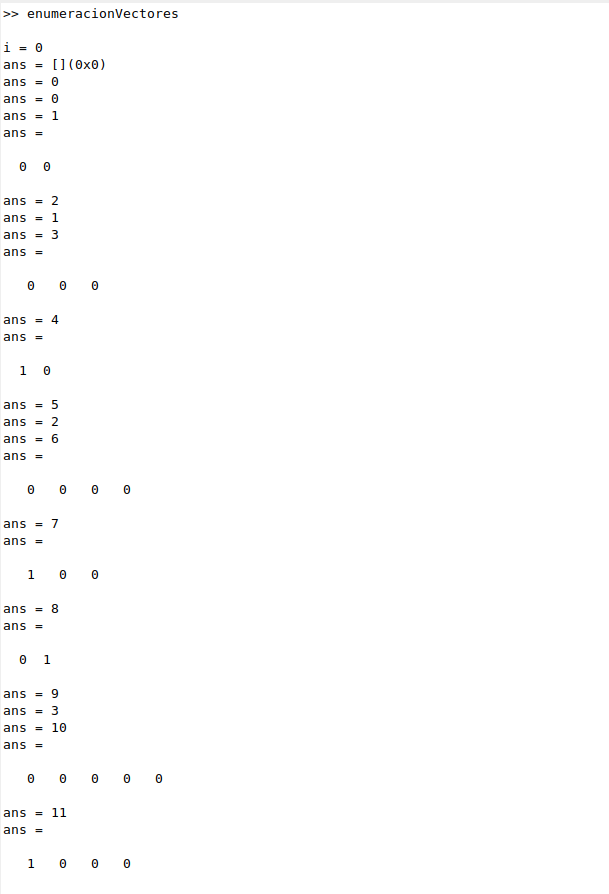
\includegraphics[scale=0.5]{Vectores}



\section*{Actividad 3}
Create an Octave script that enumerates all the WHILE programs.
\begin{verbatim}
i = 0
while (true)
  N2WHILE(i)
  i++
endwhile
\end{verbatim}
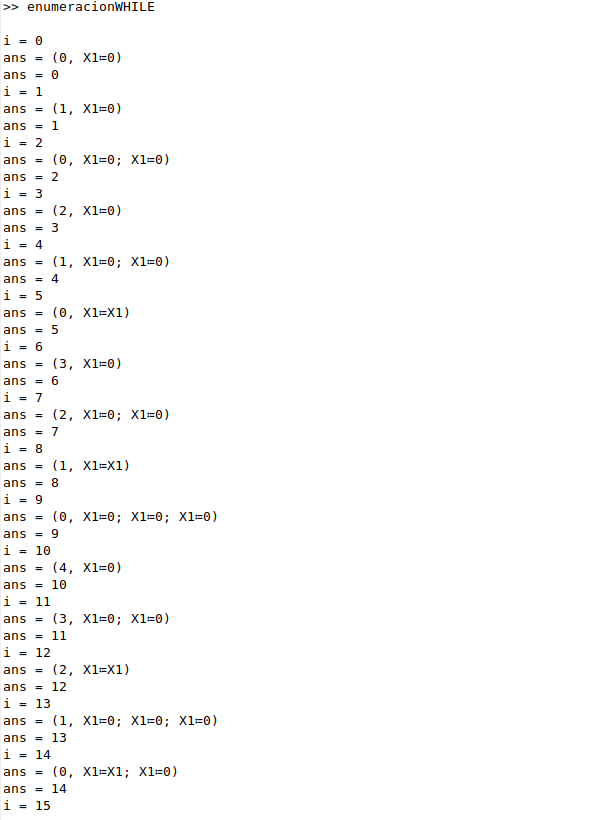
\includegraphics[scale=0.5]{While}

\end{document}